
\documentclass{article}
\pdfpagewidth=8.5in
\pdfpageheight=11in
\usepackage{ijcai20}

% Use the postscript times font!
\usepackage{times}
\renewcommand*\ttdefault{txtt}
\usepackage{soul}
\usepackage{url}
\usepackage[hidelinks]{hyperref}
\usepackage[utf8]{inputenc}
\usepackage[small]{caption}
\usepackage{graphicx}
\usepackage{amsmath}
\usepackage{booktabs}
\usepackage{lipsum}
\urlstyle{same}

\usepackage[ruled,vlined,linesnumbered]{algorithm2e}
\usepackage{subcaption}
\usepackage{tikz}
\usepackage{pgfplots}
\usepgfplotslibrary{fillbetween}

% Layers
\pgfdeclarelayer{nodelayer}
\pgfdeclarelayer{edgelayer}
\pgfsetlayers{edgelayer,nodelayer,main}

% Node styles
\tikzstyle{box}=[fill=white, draw=black, shape=rectangle, minimum width=2cm, minimum height=0.5cm]
\tikzstyle{circle}=[fill=white, draw=black, shape=circle]

% Edge styles
\tikzstyle{directed edge double}=[<->]
\tikzstyle{directed edge}=[->]

% Plot size
\pgfplotsset{width=\textwidth/2.6,compat=newest} 


\let\OLDthebibliography\thebibliography
\renewcommand\thebibliography[1]{
  \OLDthebibliography{#1}
  \setlength{\parskip}{0pt}
  \setlength{\itemsep}{0pt plus 0.3ex}
}

\newcommand{\citationneeded}{\textsuperscript{[citation needed]}}
\newcommand\floor[1]{\lfloor#1\rfloor}
\newcommand\ceil[1]{\lceil#1\rceil}

\title{Message efficient Byzantine Reliable Broadcast protocols on known topologies}

\author{
Tim Anema$^1$\and
J{\'e}r{\'e}mie Decouchant$^1$
\affiliations
$^1$TU Delft\\
\emails
\{t.p.d.anema\}@student.tudelft.nl,
\{j.decouchant\}@tudelft.nl
}


\begin{document}
\maketitle

\begin{abstract}
TODO: abstract

\lipsum[1]
% The abstract should be short and give the overall idea:
% what is the background, the research questions, what is contribution, and what are the main conclusions.
% It should be readable as a stand-alone text (preferably no references to the paper or outside literature).
\end{abstract}

\section{Introduction}
% \begin{itemize}
% \item Introduce the topic and explain why it is important (motivation!).

% \item Relate to the most relevant existing work from the literature (use BibTeX) \cite{example}, explain their contributions, and (critically) indicate what is still unanswered. 


% \item Explain what the research questions for this work are. 
% This usually is a subset of the unanswered questions. 

% \item Summarize the main contributions/conclusions of this research.
% NB: Make sure the title of the paper is a good match to the main research question / contribution / conclusion.

% \item Briefly indicate how the rest of the paper fits together to answer the research question.
% \end{itemize}

% For a longer research paper, a section with more elaborate discussion of the literature may follow, but for short (conference) submissions, this is often included in the introduction.


Distributed systems are at the heart of our everyday lives. These systems consist of autonomous processes that communicate with a subset of other processes in order to coordinate their efforts. This means that these systems have to be robust against arbitrary behaviour that some faulty or malicious nodes might exhibit. Fault-tolerant distributed communication algorithms are being used in practice to give this guarantee. 

The Byzantine fault model is often used to describe these fault-tolerant systems~\citationneeded. In this model there are two types of processes: correct processes which follow their programming faithfully, and Byzantine processes which exhibit arbitrary behaviour which can consist of altering messages, creating new ones, or dropping messages all together.

There are several solutions to this problem, all of which make different assumptions and differ in their guarantees. An example of this is Dolev's \textit{reliable communication} (RC) algorithm~\cite{dolev}, which assumes a $2f+1$-connected network. Another example is Bracha's double echo authenticated broadcast~\cite{bracha}, which assumes a fully-connected network. The state-of-the-art solution for \textit{Byzantine Reliable Broadcasts} (BRB) described in \cite{bracha-dolev} and improved in \cite{bonomi2021practical} relies on an optimized combination of Dolev's RC algorithm \cite{bonomi2019multihop} and Bracha's double echo authenticated broadcast.

This research will focus on optimizing Dolev, Bracha, and Bracha-Dolev by minimizing the amount of redundant messages transmitted when the topology of the network is known to all processes. While the problem of reducing the amount of messages has been discussed in several papers, they focus on unknown network topologies~\cite{dolev-improvement,bonomi2019multihop,bonomi2021practical}, introduce cryptography and/or \textit{public-key infrastructure} (PKI)~\cite{signatures-crypo-1,pki-crypto-2}, or use trusted nodes~\cite{using-tee}. Focusing on the case where the network topology is known to all processes is worth investigating, as this is a realistic use-case and might allow for more optimizations. In addition to this, other papers have shown ways to reconstruct the topology~\cite{topology-discovery}, which makes it possible to use the optimizations in this paper for previously unknown topologies.
Even though the aforementioned papers do not assume a known network, most of their optimizations also apply.

TODO: discuss results (around 1 paragraph)

TODO: discuss paper structure (around 1 paragraph)

\subsection*{Related work}
The idea of reliably reaching an agreement in the presence of faulty or malicious processes was first introduced by Lampert et al.~\citationneeded, and was named the \textit{Byzantine Agreement}. The network tolerance to faults can represented as $f$, which represents the amount of Byzantine processes that can be present before correct processes can no longer reliably communicate with each other. One can imagine this number heavily depends on the connectivity, i.e. the amount of nodes that can fail before the network is partitioned, of the network. A simple connected (1-connected) network will already be partitioned when a single Byzantine process exists, while a fully connected network (n-connected) can sustain more Byzantine nodes. Pease et al. proved that there exists a tight upperbound for $f$ in these networks, namely $f < \floor{N/3}$~\citationneeded.

When a network is partially connected, Dolev showed that processes can still communicate in the presence of $f$ Byzantine nodes when the network is at least $2f+1$-connected~\cite{dolev}. In this solution a message is flooded over the network, therefore following at least $2f+1$ vertex-disjoint paths. Since authenticated links\footnote{Authenticated links guarantee messages sent over a link originate from the complementing process} are assumed in this solution, every process can append the transmitter of a message to a header representing the message path. A process delivers a message when it has received the same payload data over $f+1$ vertex-disjoint paths. Note that this means it is possible for a Byzantine sender to cause a single correct process to deliver a message, violating the basic principles of a broadcast.

Bracha described the \textit{authenticated double echo} protocol~\cite{bracha} for fully connected networks, which gives the additional guarantee that either every correct process will deliver a message or none will. This protocol uses three phases -namely \textit{send}, \textit{echo}, and \textit{ready}- to coordinate the global acceptance of a message $m$.

In their original versions, both protocols are less than practical. In the case of Dolev, the worst-case message and computational complexity is high, making it impractical for large ($n=100$) networks. While Bracha is computationally less expensive, it requires a fully connected network, reducing its applicability in regular networks.

Bonomi et al.~\cite{bonomi2019multihop} introduced several improvements to Dolev's original protocol, considerably improving its average message complexity. These modifications make Dolev more practical for use in general networks, even though the complexity of delivery verification is still high. The following modifcations were introduced:
\begin{itemize}
    \item If process $p$ receives a message $m$ directly from the source $s$ over an authenticated link, then $p$ will directly deliver the message.
    \item If a message $m$ has been delivered by a process $p$, then it can discard all related Dolev paths and instead use an empty path when relaying.
    \item Process $p$ only relays messages to neighbours that have not yet delivered it.
    \item If process $p$ receives an empty path from a neighbour $q$, then it no longer has to relay and analyse messages to and from $q$.
    \item Process $p$ stops relaying messages after its contents have been delivered and the empty path has been forwarded.
\end{itemize}

Wang and Wattenhofer~\cite{bracha-dolev} introduced a new protocol, which combines Bracha and Dolev in order to use a protocol designed for a fully connected network (e.g. Bracha's protocol) on a k-connected (where $k < |V|$) network. More recently, Bonomi et al.~\cite{bonomi2021practical} introduced several novel improvements to this protocol and combined it with an optimized version of Dolev's RC protocol~\cite{dolev-improvement,bonomi2019multihop}. Their experiments showed promising results, and the possibility of extending these to other protocols exists. Let us recall their modifications with their original identification:
\begin{itemize}
    \item \textbf{MBD.1}: Limit the payload data transmission by associating local IDs to payload data. When process $p$ sends payload data it includes a generated local ID, and only uses that local ID for further transmissions of the same payload data. 
    \item \textbf{MBD.2}: When process $p$ receives Bracha's \textit{send} message it will not propogate it, but instead switch to regular \textit{echo} messages. Other processes will implicitly receive a \textit{send} message when they receive an \textit{echo} message.
    \item \textbf{MBD.3}: When process $p$ needs to transmit two echo messages with an empty path to the same neighbour, the messages are merged into a single \textit{echo\_echo} message. This situation can occur when a process transmits an \textit{echo} message after a Dolev-deliver, and another \textit{echo} message because of said Dolev-deliver with echo amplification\footnote{In addition to ready amplification~\citationneeded, echo amplification can also applied}.
    \item \textbf{MBD.4}: Similar to \textit{echo\_echo} messages, a process can also transmit a \textit{echo\_ready} message when a Dolev-deliver causes an additional echo, and a transition to the \textit{ready} state.
    \item \textbf{MBD.6}: When process $p$ Dolev-delivers a \textit{ready} message originating from process $q$, echo messages originating from $q$ can be ignored by $p$.
    \item \textbf{MBD.7}: When process $p$ Bracha-delivers a message $m$, it can ignore and discard all \textit{echo} messages related to $m$.
    \item \textbf{MBD.8}: When process $p$ has Dolev-delivered a \textit{ready} message from neighbouring process $q$, it can abstain from sending \textit{echo} messages to $q$.
    \item \textbf{MBD.9}: TODO: summarize this one
    \item \textbf{MBD.10}: TODO: summarize this one
    \item \textbf{MBD.11}: Use a subset of process of size $\ceil{\frac{N+f+1}{2}} + f$ and $3f+1$ to complete the \textit{echo} and \textit{ready} phase, respectively.
    \item \textbf{MBD.12}: If a source $s$ has more than $2f+1$ neighbours, it can transmit the \textit{send} message to only $2f+1$ of them instead of all.
\end{itemize}

TODO: talk about other solutions (signatures, trusted nodes, HotStuff BFT) and how they could be applied.


\section{System model and problem statement}
\label{system-model}
% Choose one that fits your research best:
% \subsection{Methodology}
% Typically in general research articles, the second section contains a description of the research methodology, explaining what you, the researcher, is doing to answer the research question(s), and why you have chosen this method.
% For purely analytical work this is a description of the data collection or experimental setup on how to test the hypothesis, with a motivation.
% In any case this section includes references to necessary background information.

% \subsection{Formal Problem Description}
% For some types of work in computer science the methodology is standard: analyze the problem (e.g., make assumptions and derive properties), present a new algorithm and its theoretical background, proving its correctness, and evaluate unproven aspects in simulation.
% Then an explanation of the methodology is often omitted, and the setup of the evaluation is part of a later section on the evaluation of the ideas.\footnote{This already shows that there is no single outline to be given for all papers.}
% In this case, explain relevant concepts, theory and models in this section (with references) and relate them to your research question.
% Also this section then typically contains a more precise, formal description of the problem.

% Do not forget to give this section another name, for example after the problem you are solving.

A distributed model is defined by a set $\Delta=\{p_1, p_2,...,p_N\}$ of N processes, uniquely identified by an ID $i$. In the Byzantine fault-model it is assumed that there are at most $f < \floor{N/3}$ Byzantine nodes, which can exhibit arbitrary behaviour. 

Furthermore, the processes are connected by a network which can be represented by an undirected graph $G=(V,E)$. In this graph every vertex represents a process $p_i$, such that $p_i \in \Delta$, which means $V=\Delta$ for all intents and purposes. It follows that the edges represent the communication links between nodes.
Processes $p_i, p_j \in \Delta$ have a direct communication link if there exists an edge $(v_i, v_j) \in E$, which they can use to directly communicate with each other. If there exists no such link, they will have to rely on other processes to relay their messages. We assume these links are authenticated, i.e. messages delivered at $p_i \in \Delta$ via edge $(v_i, v_j) \in E$ are guaranteed to originate from $p_j$, and vice-versa. In addition to this, the links are reliable, i.e. messages will always arrive at $p_i$ if and only if $p_j$ sent them over edge $(v_i, v_j)$. However, there is no delivery time guarantee, so a link can be synchronous or asynchronous. Graph $G$ is known to all processes, and so are the IDs for every process. Furthermore, it is assumed the network is static, i.e. the network topology does not change, and the network lives for a considerable amount of time.

In order to send message data to others, processes can add information to the message header, which can be used to uniquely identify the message and add protocol specific information.

A Byzantine Reliable Broadcast (BRB) protocol guarantees the following properties:\\
(i) \textbf{Validity}: If process $p_i \in \Delta$ broadcasts message $m$, then every correct process $p_j \in \Delta$ delivers $m$ at some point.\\
(ii) \textbf{No duplication}: A message $m$ broadcast by process $p_i \in \Delta$ is not delivered more than once by every correct process $p_j \in \Delta$.\\
(iii) \textbf{Integrity}: If process $p_j \in \Delta$ delivers message $m$ with sender $p_i$, process $p_i$ has broadcast $m$ in the past.\\
(iv) \textbf{Agreement}: If process $p_i \in \Delta$ delivers message $m$, then $m$ will eventually be delivered by every correct process $p_j \in \Delta$.

% \begin{itemize}
%     \item \textbf{Validity}: If process $p_i \in \Delta$ broadcasts message $m$, then every correct process $p_j \in \Delta$ delivers $m$ at some point.
%     \item \textbf{No duplication}: A message $m$ broadcast by process $p_i \in \Delta$ is not delivered more than once by every correct process $p_j \in \Delta$.
%     \item \textbf{Integrity}: If process $p_j \in \Delta$ delivers message $m$ with sender $p_i$, process $p_i$ has broadcast $m$ in the past.
%     \item \textbf{Agreement}: If process $p_i \in \Delta$ delivers message $m$, then $m$ will eventually be delivered by every correct process $p_j \in \Delta$.
% \end{itemize}

We will be introducing improvements to both Dolev~\cite{dolev}, Bracha~\cite{bracha}, and Bracha-Dolev~\cite{bracha-dolev}, which make different assumptions about the network $G$ and the BRB guarantees.

Dolev assumes a network $G$ which is at least $2f+1$-connected, i.e. there are at least $2f+1$ vertex-disjoint paths from every vertex $v_i \in V$ to every vertex $v_j \in (V - \{v_i\})$. Furthermore, Dolev assumes Reliable Communication (RC) which guarantees the same properties as BRB, except for the agreement property.

Bracha assumes a fully connected network $G$, i.e. for every pair $v_i,v_j \in V$ there exists an edge $(v_i, v_j) \in E$. Unlike Dolev, Bracha guarantees all BRB properties.

Bracha-Dolev is a combination of the previous protocols, and assumes a $2f+1$-connected network $G$, while giving all BRB guarantees.

\subsection*{Background}
In this section we will explain Dolev's and Bracha's protocols, and how they can be combined intro Bracha-Dolev.

\subsubsection{Dolev}
Dolev's protocol provides reliable communication when the network has authenticated links and is at least $2f+1$-connected.

When a message traverses the network, processes leverage the authenticated links to build a traversal path for each message. Said paths have two purposes: avoiding transmitting loops and message verification. 
The former is at play when processes relay messages to their neighbours; a message is forwarded to all neighbours, except to the transmitter and processes which are already present in the path. This is required in order to avoid messages circulating through the network indefinitely.
The paths are also used for verification; a message is delivered whenever it has been received over $f+1$ disjoint paths.

The basis for the correctness for Dolev's protocol lies in Menger's theorem~\cite{menger} which shows there exist $2f+1$ disjoint paths if a network is $2f+1$-connected, and the fact that at most $f$ of those paths can contain one or more Byzantine processes. This follows from the fact that a single process can only be in a single path, otherwise said path would not be disjoint, so the worst case is that all $f$ Byzantine processes are spread over all the $2f+1$ disjoint paths, which leaves $f+1$ paths not containing a Byzantine process.

There are multiple ways to implement the verification, but the problem is often reduced to a max flow problem or a minimum vertex cut problem. We will elaborate on the first option. In this case paths are modeled as a flow network where every edge has a capacity of one. The maximum flow through the network from source $p_j$ to sink $p_i$ is then equal to the amount of disjoint paths. The max flow can be found with the Ford-Fulkerson algorithm~\cite{ford_fulkerson} for example.
Pseudocode for Dolev's protocol is provided in Algorithm~\ref{background:dolev}.

\begin{algorithm}
  \DontPrintSemicolon
  \SetKwFunction{DInit}{Init}
  \SetKwProg{Fn}{On event}{:}{}
  \Fn{\DInit}{
        delivered = False\;
        paths = $\emptyset$\;
  }
  
  \SetKwFunction{DRecv}{Receive}
  \Fn{\DRecv{$p_{recv}$, $m$, $path$}}{
        $path$ = $path \cup \{p_{recv}\}$\;
        \ForAll{$p_j \in neighbours - path$}{
            transmit($p_j$, $m$, $path$)\;
        }
  
        paths.add($path$)\;

        \uIf{paths contains $f+1$ node-disjoint paths to the origin \textbf{and} delivered = False}{
            deliver($m$)\;
            delivered = True\;
        }
  }
  
  \SetKwFunction{DBrd}{Broadcast}
  \Fn{\DBrd{$m$}}{
        deliver($m$)\;
        delivered = True\;
            
        \ForAll{$p_j \in neighbours$}{
            transmit($p_j$, $m$, $\emptyset$)\;
        }
  }
 \caption{Dolev's Reliable Communication algorithm}
 \label{background:dolev}
\end{algorithm}

\subsubsection{Bracha}
Unlike Dolev's protocol, Bracha's protocol requires a fully connected network while giving all BRB guarantees. The protocol has three phases: \textit{send}, \textit{echo}, and \textit{ready}.

When a process wants to broadcast a message it sends the payload in a \textit{send} message to all processes, including itself. When a process receives a \textit{send} messages, it responds by transmitting an \textit{echo} message to all processes with the corresponding content. Every process then waits for a quorum of \textit{echo} messages, which is $\ceil{\frac{N+f+1}{2}}$. 
After this quorum has been reached, or $f+1$ \textit{ready} messages have been received, a process will transmit its own \textit{ready} message to all processes. Finally, a message will be delivered when $2f+1$ corresponding \textit{ready} messages have been received, as can be seen in Algorithm~\ref{background:bracha}.

\begin{algorithm}[h]
  \DontPrintSemicolon
  \SetKwFunction{BInit}{Init}
  \SetKwProg{Fn}{On event}{:}{}
  \Fn{\BInit}{
        sentEcho = sentReady = delivered = False\;
        echos = readys = $\emptyset$\;
  }
  
  \SetKwFunction{BRecvEcho}{ReceiveEcho}
  \Fn{\BRecvEcho{$p_{recv}$, $m$}}{
        \uIf{\textbf{not} sentEcho}{
            \ForAll{$p_j \in neighbours$}{
                transmit($p_j$, $m$, ECHO)\;
            }
            
            sentEcho = True\;
        }
        
        echos.add($p_{recv}$)\;

        \uIf{len(echos) $\ge$ $\ceil{\frac{N+f+1}{2}}$ \textbf{and not} sentReady}{
            \ForAll{$p_j \in neighbours$}{
                transmit($p_j$, $m$, READY)\;
            }
            
            sentReady = True\;
        }
  }
  
  \SetKwFunction{BRecvReady}{ReceiveReady}
  \Fn{\BRecvReady{$p_{recv}$, $m$}}{
        readys.add($p_{recv}$)\;

        \uIf{len(readys) $\ge f+1$ \textbf{and not} sentReady}{
            \ForAll{$p_j \in neighbours$}{
                transmit($p_j$, $m$, READY)\;
            }
            
            sentReady = True\;
        }
        
        \uIf{len(readys) $\ge 2f+1$ \textbf{and not} delivered}{
            deliver($m$)\;
            delivered = True\;
        }
  }
  
  \SetKwFunction{BBrd}{Broadcast}
  \Fn{\BBrd{$m$}}{
        \ForAll{$p_j \in neighbours$}{
            transmit($p_j$, $m$, SEND)\;
            transmit($p_j$, $m$, ECHO)\;
        }
  }
 \caption{Bracha's authenticated double echo algorithm}
 \label{background:bracha}
\end{algorithm}

\subsubsection{Bracha-Dolev}
Dolev's and Bracha's protocol can be combined to achieve BRB guarantees in a multi-hop network, as described in \cite{bracha-dolev}. 

This works by layering the two protocols, where Dolev's protocol forms the bottom layer. This means every Bracha broadcast is replaced by a Dolev broadcast, and every Bracha receive by a Dolev deliver. This process is shown in figure~\ref{background:bracha-dolev}.

By layering Bracha and Dolev, the latter emulates a fully connected network by enabling the former to reliably reach all processes. However, this means the message complexity of both protocols %, $\mathcal{O}(n^2)$ and $\mathcal{O}(n!)$ respectively,% 
is essentially multiplied.

Instead of simply layering the two protocols, a cross-layer version~\cite{bonomi2021practical} can be used which allows for greater optimization. For comparison, this version can be seen in figure~\ref{background:bracha-dolev}.

\begin{figure}
    \centering
    \begin{subfigure}{.2\textwidth}
      \centering
      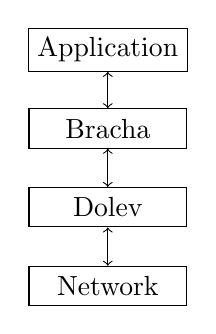
\begin{tikzpicture}
        	\begin{pgfonlayer}{nodelayer}
        		\node [style=box] (0) at (-4.25, 6.25) {Application};
        		\node [style=box] (1) at (-4.25, 5.25) {Bracha};
        		\node [style=box] (2) at (-4.25, 4.25) {Dolev};
        		\node [style=box] (3) at (-4.25, 3.25) {Network};
        	\end{pgfonlayer}
        	\begin{pgfonlayer}{edgelayer}
        		\draw [style=directed edge double] (0) to (1);
        		\draw [style=directed edge double] (1) to (2);
        		\draw [style=directed edge double] (2) to (3);
        	\end{pgfonlayer}
        \end{tikzpicture}
    %   \caption{Layering Bracha and Dolev forms the basis for Bracha-Dolev}
    \end{subfigure}
    \begin{subfigure}{.2\textwidth}
      \centering
      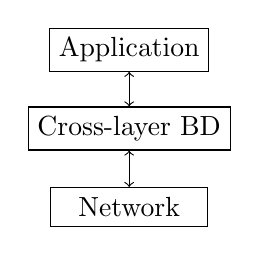
\begin{tikzpicture}
        	\begin{pgfonlayer}{nodelayer}
        		\node [style=box] (0) at (-4.25, 6.25) {Application};
        		\node [style=box] (1) at (-4.25, 5.25) {Cross-layer BD};
        		\node [style=box] (2) at (-4.25, 4.25) {Network};
        % 		\node [style=none] (3) at (-4.25, 3.25) {};
        	\end{pgfonlayer}
        	\begin{pgfonlayer}{edgelayer}
        		\draw [style=directed edge double] (0) to (1);
        		\draw [style=directed edge double] (1) to (2);
        	\end{pgfonlayer}
        \end{tikzpicture}
    %   \caption{A cross-layer combination can be used to improve performance~\cite{bonomi2021practical}}
    \end{subfigure}
    \caption{Bracha-Dolev can be implemented by simply layering the two protocols or by using a cross-layer protocol~\cite{bonomi2021practical}}
    \label{background:bracha-dolev}
\end{figure}

\subsection*{Reducing the amount of messages}
While all mentioned protocols work well in their designed environments, there is naturally a substantial amount of redundant work.

In the case of Dolev, for example, the network is being flooded with the same message in order to reach all processes over at least $f+1$ vertex-disjoint paths. However, if the network is overprovisioned, i.e. the network is $k$-connected where $k > 2f+1$, the message will take more paths than strictly necessary. In addition to this, processes will send the message to (almost) all neighbours leading to overlapping paths. Even though recent improvements have reduced the amount of required messages 
fr%om $\mathcal{O}(n!)$ to nearly $\mathcal{O}(n)$~\cite{bonomi2019multihop}
, it is possible this can still be reduced if processes have knowledge of the network topology.

For Bracha there are similar inefficiencies. For example, Bracha uses all nodes to come to an agreement, while only a subset of size $\ceil{\frac{N+f+1}{2}} + f$ is needed in the \textit{echo} phase and a smaller subset of size $3f+1$ for the final \textit{ready} phase.

The optimizations can be combined and applied to Bracha-Dolev, also reducing the amount of required messages for that protocol.

The aim of this paper is to reduce the amount of messages being transmitted and network usage even further, assuming the processes know the network topology. In addition to this, it might be possible to improve the delivery complexity of Dolev in the process by taking advantage of the fact that messages will traverse fixed paths. Furthermore, while the general process for handling known topologies for Dolev has been described in the original paper~\cite{dolev}, no actual implementation has been provided, which is something this paper will also do.

% \section{Your contribution}
% In computer science typically the third section contains an exposition of the main ideas, for example the development of a theory, the analysis of the problem (some proofs), a new algorithm, and potentially some theoretical analysis of the properties of the algorithm.

% Do not forget to give this section another name, for example after the method or idea you are presenting.

% Some more detailed suggestions for typical types of contributions in computer science are described in the following subsections.

% \subsection*{Experimental work}
% In this case, this section will mostly contain a description of the methods/algorithms you will be comparing. Although not all methods need to be described in detail (providing appropriate references are available), make sure that you reveal sufficient details to a reader not familiar with these methods to: a) obtain a high-level understanding of the method and differences between them, and b) understand your explanation of the results.

% \subsection*{Improvement of an idea}
% In this case, you would need to explain in detail how the improvement works. If it is based on some observation that can be proven, this is a good place to provide that proof (e.g., of the correctness of your approach). 

\section{Dolev on known topologies}
\label{contr-dolev}
In this section we will describe the algorithms required to leverage the potential of topology knowledge, how Dolev can be modified to run on known topologies, and \textbf{7} novel modifications to the resulting protocol.

\subsection{Finding k-disjoint paths}
In order to build a routing table, one has to find $k$ vertex-disjoint paths to every $p_i \in \Delta$. Formally this problem is known as the \textit{min-sum disjoint paths problem}.

A straight-forward solution would be to repeatedly find the shortest path, remove the edges in the path, and repeat this process $k$ times. However, even though this algorithm would work on most graphs, there exist so-called \textit{trap topologies} for which this algorithm would fail to find a solution. In said topologies there exists a path with a minimal sum, which traverses multiple disjoint paths, effectively blocking off more disjoint paths than needed. An example of a trap topology can be found in figure~\ref{contr:trap-topology}. In this example the path \textit{a-c-b-d} would be chosen over \textit{a-b-d} and \textit{a-c-d} by this naive algorithm.


\begin{figure}[h]
    \centering
    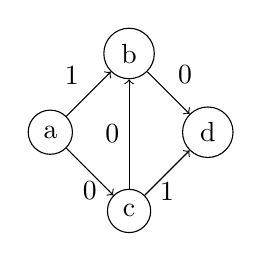
\begin{tikzpicture}
    	\begin{pgfonlayer}{nodelayer}
    		\node [style=circle] (0) at (0, 0) {a};
    		\node [style=circle] (1) at (1, 1) {b};
    		\node [style=circle] (2) at (1, -1) {c};
    		\node [style=circle] (3) at (2, 0) {d};
    	\end{pgfonlayer}
    	\begin{pgfonlayer}{edgelayer}
    		\draw [style=directed edge] (0) to node [below] {0} (2);
    		\draw [style=directed edge] (2) to node [below] {1} (3);
    		\draw [style=directed edge] (0) to node [auto] {1} (1);
    		\draw [style=directed edge] (1) to node [auto] {0} (3);
    		\draw [style=directed edge] (2) to node [auto] {0} (1);
    	\end{pgfonlayer}
    \end{tikzpicture}
    \caption{In this example there exist two paths from $a$ to $d$, but only one would be found by a naive shorted path algorithm}
    \label{contr:trap-topology}
\end{figure}

A solution which is able to handle trap topologies was introduced by Bhandari~\cite{bhandari}. This algorithm finds $k$ edge-disjoint paths in a directed weighted graph by repeatedly finding the shortest path and inverting the resulting edges. An edge is inverted by simply reversing its direction and multiplying its weight by $-1$. If there already exists a reverse edge for the edge being inverted, the existing edge is replaced. If the edge being inverted has already been inverted once, it can be simply discarded instead.
To find the result, all complementing edges are removed from the set with all edges in the paths. The final paths can then easily be retrieved from the resulting sets, as every edge will only have two or less matching edges.

Note that this algorithm only returns $k$ edge-disjoint paths, not $k$ vertex-disjoint paths. This problem can be solved by applying a process called \textit{vertex splitting}, which as the name implies splits every vertex with the exception of source and sink into two distinct vertices. 
A vertex is split into an 'in' vertex, and an 'out' vertex. Every incoming edge will be directed to the former, while every outgoing edge will be directed to the latter. The two vertices are connected by a directed edge with a weight of zero from the 'in' vertex to the 'out' vertex. This process is visualized in figure~\ref{contr:node-splitting}. Note that this change forces every path which uses a vertex to use the interconnecting edge, limiting the amount of times every vertex can be used to one. This means the algorithm will now find $k$ vertex-disjoint paths.

\begin{figure}[h]
    \centering
    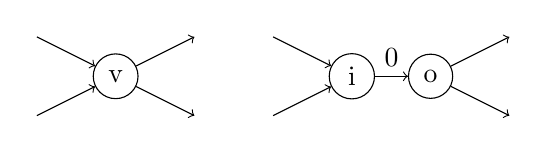
\begin{tikzpicture}
    	\begin{pgfonlayer}{nodelayer}
    		\node [style=circle] (0) at (0, 0) {v};
    		\node (2) at (-1, 0.5) {};
    		\node (3) at (-1, -0.5) {};
    		\node (4) at (1, 0.5) {};
    		\node (5) at (2, 0.5) {};
    		\node (6) at (2, -0.5) {};
    		\node [style=circle] (7) at (3, 0) {i};
    		\node [style=circle] (8) at (4, 0) {o};
    		\node (9) at (5, 0.5) {};
    		\node (10) at (1, -0.5) {};
    		\node (11) at (5, -0.5) {};
    	\end{pgfonlayer}
    	\begin{pgfonlayer}{edgelayer}
    		\draw [style=directed edge] (2.center) to node [auto] {} (0);
    		\draw [style=directed edge] (3.center) to (0);
    		\draw [style=directed edge] (0) to (4.center);
    		\draw [style=directed edge] (5.center) to (7);
    		\draw [style=directed edge] (6.center) to (7);
    		\draw [style=directed edge] (8) to (9.center);
    		\draw [style=directed edge] (0) to (10.center);
    		\draw [style=directed edge] (8) to (11.center);
    		\draw [style=directed edge] (7) to node [auto] {0} (8);
    	\end{pgfonlayer}
    \end{tikzpicture}
    \caption{Vertex splitting visualized}
    \label{contr:node-splitting}
\end{figure}

In order to build the full routing table, this process has to be completed for every process, resulting in $(n-1) * (2f+1)$ paths which will reach every process over $2f+1$ node-disjoint paths.

The pseudocode for the $k$-disjoint path solver can be found in Algorithm~\ref{contr:disjoint-path}. We use the Shortest Path Faster Algorithm or SPFA~\cite{spfa-moore,spfa-fanding}, which is a queue-based Bellman-Ford~\cite{bf-bellman,bf-ford} variation to find the shortest path in our paper, but any algorithm can be used which is capable of handling negative weights. In order to build a full routing table based on our disjoint path solver, one only has to vary the $t$ parameter, which is essentially the target process. The full table can be build by iterating over all processes for $t$.

\begin{algorithm}[h]
  \DontPrintSemicolon
  \SetKwFunction{DisPaths}{DistjointPaths}
  \SetKwProg{Fn}{func}{:}{}
  \Fn{\DisPaths{$g$, $s$, $t$, $k$}}{
        edges = DisjointEdges($g$, $s$, $t$, $k$)\;
        filtered = FilterCounterparts(edges)\;
        
        \textbf{return} BuildPaths(filtered, $s$, $t$, $k$)\;
  }
  
  \SetKwFor{RepTimes}{repeat}{times}{end}
  \SetKwFunction{DisEdges}{DisjointEdges}
  \Fn{\DisEdges{$g$, $s$, $t$, $k$}}{
        split = VertexSplitting($g$)\;
        result = $\emptyset$\;
        \RepTimes{k}{
            path = ShortestPath($s$, $t$, split)\;
            
            \ForAll{$e \in path$}{
                result.add($e$)\;
                InverseEdge(split, $e$)\;
            }
        }
        
        \textbf{return} result\;
  }
  
  \SetKwFunction{FilterCounter}{FilterCounterparts}
  \Fn{\FilterCounter{$edges$}}{
        drop = result = $\emptyset$\;
            
        \ForAll{$(f,t) \in edges$}{
            drop.add($(t,f)$)\;
        }
        
        \ForAll{$e \in edges$}{
            \uIf{\textbf{not} drop.contains($e$)}{
                result.add($e$)\;
            }            
        }
        
        \textbf{return} result\;
  }
  
  \SetKwFunction{BuildPaths}{BuildPaths}
  \Fn{\BuildPaths{$edges$, $s$, $t$}}{
        result = $\emptyset$\;
            
        \ForAll{$(f,e) \in edges$}{
            \uIf{$f = s$}{
                path = $\emptyset$\;
                
                \While{\textbf{not} $e$ = $t$}{
                    path.add($(f,e)$)\;
                    $(f,e)$ = Next($e$)\;
                }
                
                path.add($(f,e)$)\;
                result.add(path)\;
            }
        }
        
        \textbf{return} result\;
  }
 \caption{Disjoint path solver algorithm}
 \label{contr:disjoint-path}
\end{algorithm}

\subsection{Modifying Dolev}
\label{contr:modifying-dolev}
We can distinguish between two options for the routing table in a modified verion of Dolev's protocol. 
In one version a process only computes its own routing table, while in the other version every process calculates the routing table of every other process including its own. The former is less computationally expensive, but the latter requires less information to be transmitted, since the desired path needs to be included in the message header for the former version to work. The latter option also allows for trivial message verification, as every process is aware of the paths another process will use to communicate. 

% In one version every process only uses the edge weights without any modifications to calculate the routing table. Note that this results in routing tables where $paths(p_i, p_j) == reverse\_paths(p_j, p_i)$ where $p_i, p_j \in \Delta$, i.e. for every pair of arbitrary processes $p_i$ and $p_j$ the paths of $p_i$ to $p_j$ all have reverse paths\footnote{Let us recall that a reverse path is simply a path traversed backwards} in the set of paths from $p_j$ to $p_i$.
% Another version allows for individual processes to make changes to their edge weights, so messages might traverse different paths from $p_i$ to $p_j$ than from $p_j$ to $p_i$.

% The former allows for trivial message verification as every node is aware of the paths a message should traverse. However, processes can not deviate from the original edge weights, which might be undesirable for future improvements. The second option allows processes to change weights and have dynamic routing tables, but does require more care when verifying messages.

% In both cases there is still another decision to make. Should every process compute the routing tables of all other processes, or should every process only compute their own routing table? Both cases are valid, but they differ in their computational complexity and their bandwidth usage. Computing every routing table is a computationally expensive operation, but allows for information to be removed from the messages, reducing the amount of required bandwidth.

% In this paper we have opted for the protocol where every process only computes its own routing table and they are allowed to change edge weights.

In this paper we have opted for the protocol where every process has access to every routing table in order to decrease the message size, as will be discussed later.

\subsubsection{Modifications}
The protocol is changed in several places, in order to maximally leverage topology knowledge. 

The messages do not change significantly, all original information is retained.

The message verification is simplified greatly, as every message path can now be simply compared to the corresponding routing table entry. If no matching entry exists for the given origin,, the message is discarded. Otherwise it is kept in memory. Once enough messages with identical payloads and unique paths have been received the message is delivered. This can easily achieved by creating a mapping between a message identifier, consisting of the regular Dolev identifier and the hash of the payload, and a set of paths. When the size of the set of paths is equal to $f+1$, corresponding content can be delivered.

% This version of Dolev's protocol knows two possible verification algorithms. 
% Since a process $p_i$ is initially unaware of the paths used by process $p_j$, it must fall back on basic Dolev verification, where every message has to be received over at least $f+1$ disjoint paths. This problem can be solved by modeling the paths as a flow network where every edge has a capacity of one. The maximum flow through the network from source $p_j$ to sink $p_i$ is then equal to the amount of disjoint paths. In this paper we use the Edmonds-Karp algorithm~\citationneeded to find the maximum flow through the flow network.
% When a process $p_i$ has delivered a message from $p_j$, it can save the paths used to memory. Since we assume these paths never change, they can be used to verify any message in the future in a more efficient manner. Any incoming message is accepted when it has arrived over at least $f+1$ unique paths saved in memory.

\subsection{Optimizations on routing table}
In addition to providing a base implementation for Dolev's protocol with routing, we also introduce several optimizations in order to further reduce the amount of messages transmitted. In order to avoid confusion we use the identifier \textbf{ORD.1-7} for our optimizations. This section will focus on optimizations only used while creating the routing table.

\subsubsection{ORD.1: Avoid transmitting subpaths}
When process $p$ is building its routing table, it can discard all routes which are a subpath of other routes. The messages related to said paths can be dropped without loss of information, as it is guaranteed another message will traverse the path in full.

\subsubsection{ORD.2: Use a single route for direct neighbours}
Bonomi et al.~\cite{bonomi2019multihop} showed that direct neighbours can directly deliver messages originating from the source. A similar change can be made to the routed version of Dolev's protocol, by accepting only one path to direct neighbours. We have achieved this by adding links to neighbouring processes separately prior to finding disjoint edges, which corresponds to line 2 in Algorithm~\ref{contr:disjoint-path}.

\subsubsection{ORD.3: Merge next hops when broadcasting}
When process $p$ is transmitting the initial broadcast messages, it can merge all messages which have the same first hop into a single message. This process can then be continued by all relaying nodes until only a single base message remains. This means the desired and traversed path form a pair which needs to be maintained throughout the entire network. This optimization applies to the creation of routing tables, but is also applied when processes disseminate messages as they may need to split messages.

\subsubsection{ORD.4: Reuse paths when possible}
When messages traverse the same path, processes can attempt to merge messages as explained in \textbf{ORD.3}. For this reason routes should be as similar as possible. We have achieved this by adding weights to unused edges after each iteration of the disjoint k-paths solver, which corresponds the space between line 12 and 13 in Algorithm~\ref{contr:disjoint-path}.

Additional care has to be taken when \textbf{ORD.2} is also applied, to avoid routing messages to neighbours over intermediate nodes.

\subsection{General optimizations}
This section solely focuses on optimizations which do not apply to the creation of the routing table, or are mostly applicable at message dissemination. 

\subsubsection{ORD.5: Apply delayed relaying and merging}
While \textbf{ORD.3} introduced the concept of merging messages, this is a \textit{structurally decreasing} process, i.e. the amount of wrapped messages in a single message will only decrease as the message is being relayed. The reason for this is that processes only analyse an incoming message without additional context, which means a process will process the incoming buffer sequentially and immediately relay messages when possible.
While this process is pure and has little side-effects, there are cases when using the context of other messages or delaying outbound messages is beneficial. For example, two messages with the same Dolev identifier received over two different links can be merged into a single message (similar to \textbf{ORD.3}) when they share the same next-hop. However, since these messages are handled separately the process needs to delay the former and use its context when processing the latter message.

One possible option is to only relay messages whose contents have been delivered, and keep outbound messages in a buffer which can be used to merge outbound messages. While this approach would work on some networks, a deadlock will be created when two processes are delaying messages which would otherwise cause them two deliver.

This can be avoided by detecting possible deadlocks, and then marking one of the conflicting paths as a priority path, which means processes will immediately relay it. Deadlocks can be detected by finding a pair of paths for which at least one edge in the first path and the reverse edge in the second path exists. Deciding on priority paths can be done in any way, but it's essential that at least one path is picked for every conflict. In this paper we simply decide find the processes in an overlapping section with a maximum distance and mark the path which traverses the node with the smallest ID first as a priority path, unless the other path is already marked as a priority path. An optimal solution to this problem exists, but this is outside the scope of this paper.

\textbf{Remark}
This modification introduces more latency to the protocol, as (some) messages are being held in buffers for longer amounts of time. This can be partially mitigated by applying optimizations to the deciding procedure. For example, designating paths as a priority path when all processes on the conflicting edges only have to relay that single message, since there is no other message to merge with. Another addition might be \textit{piggybacking}, which means messages in the buffer can be merged with a priority message sharing the same next hop, since the priority message will be transmitted anyways.

% In addition to using the custom buffer, it might be possible to also include the incoming network buffer for more merging possibilities. However, this is heavily dependant on the programming language and environment used, so we refrain from using the read buffer directly in this paper.

\subsubsection{ORD.6: Merging messages with identical contents}
There exist protocols where every process or a subset of processes transmits the same payload. Examples of these protocols are \textit{keepalive} or topology verification protocols. In these cases messages from different Dolev broadcasts can be merged before being relayed in a similar fashion as \textbf{ORD.5}.

The buffer from \textbf{ORD.5} can be reused as is, and the messages themselves can be retransmitted in a special wrapper message containing all information from the merged messages and a single copy of the payload.

\subsubsection{ORD.7: Reducing message size}
As discussed in Sec.~\ref{contr:modifying-dolev}, the routing information can be included in the message headers to reduce computational complexity or it can be fully precomputed to reduce the message size. When optimizing for bandwidth usage the latter is the only viable option. 

This modification ensures message headers are no larger than needed by precomputing all routing tables, which can then be used to deduce the desired paths based on the origin and the previous relay. 


\section{Bracha on known topologies}
\label{contr-bracha}
In the case of Bracha's protocol, topology knowledge is not as useful as with Dolev's protocol. This is because Bracha assumes a fully connected network, which means the topology is known anyways. The only knowledge processes gain is the weight of edges representing links between other processes. We will try to use this knowledge for our optimizations

Similar to Dolev's optimizations, we will use \textbf{ORB.1-2} to identify different optimizations.

\subsubsection{ORB.1: Implicit echo messages}
Instead of sending a \textit{send} message and an \textit{echo} message separately, a process can send a single \textit{send} message and others will interpret that as a combined \textit{send} and \textit{echo} message. Similarly, an echo or ready message will also be interpret as a \textit{send} message. This optimization is similar to \textbf{MDB.2} from~\cite{bonomi2021practical}, as that optimization converts the \textit{send} message into an \textit{echo} message after the first hop. While this is slightly different, the effects are nearly the same.

\subsubsection{ORB.2: Use minimal subset of neighbours}
Bracha's protocol requires $\ceil{\frac{N+f+1}{2}} + f$ participants in the \textit{echo} phase and $3f+1$ for the \textit{ready} phase. This means that for overprovisioned networks, i.e. networks where $f < \floor{\frac{N}{3}} - 1$, we can avoid using all processes in said phases.

This is similar to the optimization \textbf{MBD.11} from \cite{bonomi2021practical}, however we can improve overall latency by assigning a cost to every neighbour based on their outgoing edges and then making a selection. 

There are several ways to assign a cost to a process. Simple heuristics include finding the minimum sum of weights of edges used, finding the minimum sum of weights for all edges, and several other similar approaches. The optimal solution can also be computed, but that is outside of our scope. In this paper we use the simple heuristic of finding the minimum sum of weights for all edges.

Using the chosen heuristic, every process calculates a Bracha routing table which contains all \textit{echo} and \textit{ready} participants for every message origin.

In order to not add information to the message header, these participants can be precomputed by every Bracha process. These precomputed tables can then be used to find the participant sets for a given origin.

\section{Bracha-Dolev on known topologies}
\label{contr-bracha-dolev}
In this section we will describe how our previous optimizations for Dolev and Bracha can be applied to Bracha-Dolev, and additional cross-layer optimizations.

\subsection{Applying optimizations}
As Dolev is used as the lowest layer, all \textbf{ORD} optimizations can be applied as is to our improved version of Bracha-Dolev.

Bracha is used as the upper layer in Bracha-Dolev, and as such we can not directly apply \textbf{ORB.2}, since it assumes a fully connected network. However, we can use a different way of selecting processes, by simply selecting the closest processes in the network.
The other Bracha optimization, \textbf{ORB.1}, can be directly applied as it does not rely on topology knowledge.

\subsection{Optimizations}
In addition to applying all \textbf{ORD} and (modified) \textbf{ORB} optimizations, we can also apply some new modifications. These are identified by \textbf{ORBD.1-2}.

\subsubsection{ORBD.1: Using partial Dolev broadcast}
In order to take full advantage of \textbf{ORB.2} the underlying Dolev layer should avoid sending messages to processes not included in the current \textit{echo} or \textit{ready} phase. This can be achieved by using partial broadcasts, i.e. not all processes deliver a message. While this would normally violate the RC protocols of Dolev, it doesn't in this case as Bracha-Dolev as a whole still upholds the BRB guarantees.

This modification can be added by replacing the usual Dolev routing table, by two pre-computed routing tables which take the Bracha phase and message origin into account, or by reusing the regular Dolev routing table and compute the resulting routes on the fly. The former uses more memory to store all routing tables, while the latter increases the latency of the protocol.

\subsubsection{ORBD.2: Merging multiple Bracha messages}
The Dolev layer considers different Bracha messages as different payloads, which is correct. However, Bracha messages from the same Bracha-Dolev broadcast share identical payload and origin data. This can be leveraged on the Dolev layer by identifying Bracha messages belonging to the same Bracha-Dolev broadcast and merging them if possible, by utilizing the buffer created by \textbf{ORD.5}.

When merging messages, a special wrapper message is transmitted by a Dolev node, which neighbours can use to reconstruct the original messages, similar to the wrapper message in \textbf{ORD.6}

\textbf{Remark}
This optimization can likely be extended to the Bracha layer in addition to being just on the Dolev layer, to leverage topology knowledge even more. However, at this time we have no solution to this problem, but also no proof of its impossibility. This should be further explored in the future.

\section{Evaluation}
\label{eval}
% As discussed earlier, in many sciences the methodology is explained in section 2 and this section only discusses the results. 
% However, in computer science, most often the details of the evaluation setup are described here first (simulation environment, etc.).
% Very important here is that any skilled reader would be able to reproduce this setup and then obtain the same results.

% Then, results are reported in an accessible manner through figures (preferably with captions that allow them to be understood without going through the whole text), observations are made that clearly follow from the presented results.
% Conclusions are drawn that follow logically from the previous material.
% Sometimes the conclusions are in fact hypotheses, which in turn may give rise to new experiments to be validated.

% You may want to give this section another name.

In this section we will discuss the methodology we used and the results of our optimizations.

\subsection{Methodology}
For our research we implemented a small runner program in Go which uses goroutines as a process abstraction, and allocates dedicated channels which can be used as communication links. The protocol instances are instantiated by the process wrappers, and they have access to a network and an application instance, which are defined by the interfaces containing \texttt{Send(dst, m)} and \texttt{Deliver(m)} respectively. The protocols themselves provide the \texttt{Init()}, \texttt{Receive(src, m)}, and \texttt{Broadcast(m)} functions.

In addition to the original protocols and improved version of Dolev~\cite{bonomi2019multihop} and a version of Dolev with naive routing was implemented. These two versions are the baseline for Dolev and Bracha-Dolev. 
TODO: discuss bonomi 10.

We use similar graphs as used in \cite{bonomi2019multihop,bonomi2021practical}: generalized wheels, multipartite wheels, and random regular graphs. For the tests we use an AMD Ryzen 5 2600 (3.4-3.9GHz) machine. The usage of channels leads to a different throughput per machine, but their performance will not limit the tests~\citationneeded and will not affect our main measurement.

We define the latency as the time between the original broadcast and the final non-Byzantine node delivering the message. Note that the latency will not be entirely representative of the latency in a real deployment, as our simulated links have low latency which means latency is largely influenced by computing time. 

We will run the tests with varying graphs, broadcasting process, byzantine processes, and parameters $N$, $k$, $f$, such that $N \ge 3f+1$ and $k \ge 2f+1$, and report the mean and standard deviation of five tests. In most tests a single process will broadcast a single message, unless the modifications being tested include \textbf{ORD.6} as it is specifically made for the case of multiple broadcasters.

We focus on message complexity and network consumption, which is defined by the total amount of messages transmitted and total amount of bytes transmitted, respectively.

\subsection{Impact of individual optimizations}
We evaluated the impact of individual optimizations on the message complexity and network consumption. Table~\ref{eval:individual-results} summarizes our findings for every individual modification compared to its baseline. The baseline is different for each protocol: for Dolev we compare to a version with naive routing, for Bracha we compare to the original version, and for Bracha-Dolev we compare to a version of Bracha-Dolev which uses naive routing for the Dolev layer and the original Bracha implementation. For these tests random graphs were used with a size of $N=150$ and we varied the $k$ and $f$ to find out when modifications are useful. 

We will illustrate some modifications with the aforementioned configuration. TODO.

\begin{table*}
  \centering
  \resizebox{\textwidth}{!}{
\begin{tabular}{c|cc|cc|cc|cc|}
\cline{2-9}
\textbf{}                         & \multicolumn{4}{c|}{\textbf{Small payload (12B)}}                                                  & \multicolumn{4}{c|}{\textbf{Large payload (12KB)}}                                                  \\ \hline
\multicolumn{1}{|c|}{\textbf{ID}} & \textbf{Msg. red. \%} & \textbf{Useful when} & \textbf{Usage red. \%} & \textbf{Useful when} & \textbf{Msg. red. \%} & \textbf{Useful when} & \textbf{Usage red. \%} & \textbf{Useful when} \\ \hline
\multicolumn{1}{|c|}{ORD.1}       & 10\% (2\%)            & always               & 10\% (2\%)             & always               & 10\% (2\%)            & always               & 10\% (2\%)             & always               \\ \hline
\multicolumn{1}{|c|}{ORD.2}       & 10\% (2\%)            & always               & 10\% (2\%)             & always               & 10\% (2\%)            & always               & 10\% (2\%)             & always               \\ \hline
\multicolumn{1}{|c|}{ORD.3}       & 10\% (2\%)            & always               & 10\% (2\%)             & always               & 10\% (2\%)            & always               & 10\% (2\%)             & always               \\ \hline
\multicolumn{1}{|c|}{ORD.4}       & 10\% (2\%)            & always               & 10\% (2\%)             & always               & 10\% (2\%)            & always               & 10\% (2\%)             & always               \\ \hline
\multicolumn{1}{|c|}{ORD.5}       & 10\% (2\%)            & always               & 10\% (2\%)             & always               & 10\% (2\%)            & always               & 10\% (2\%)             & always               \\ \hline
\multicolumn{1}{|c|}{ORD.6}       & 10\% (2\%)            & always               & 10\% (2\%)             & always               & 10\% (2\%)            & always               & 10\% (2\%)             & always               \\ \hline
\multicolumn{1}{|c|}{ORD.7}       & 10\% (2\%)            & always               & 10\% (2\%)             & always               & 10\% (2\%)            & always               & 10\% (2\%)             & always               \\ \hline
\multicolumn{1}{|c|}{ORB.1}       & 10\% (2\%)            & always               & 10\% (2\%)             & always               & 10\% (2\%)            & always               & 10\% (2\%)             & always               \\ \hline
\multicolumn{1}{|c|}{ORB.2}       & 10\% (2\%)            & always               & 10\% (2\%)             & always               & 10\% (2\%)            & always               & 10\% (2\%)             & always               \\ \hline
\multicolumn{1}{|c|}{ORBD.1}      & 10\% (2\%)            & always               & 10\% (2\%)             & always               & 10\% (2\%)            & always               & 10\% (2\%)             & always               \\ \hline
\multicolumn{1}{|c|}{ORBD.2}      & 10\% (2\%)            & always               & 10\% (2\%)             & always               & 10\% (2\%)            & always               & 10\% (2\%)             & always               \\ \hline
\end{tabular}
    }
  \caption{Effect of modifications measured on random graphs compared to their respective protocol standard}
  \label{eval:individual-results}
\end{table*}

% \begin{table}[]
% \begin{tabular}{ll|ll|ll|ll|ll|}
% \cline{3-10}
% \multicolumn{1}{c}{\textbf{}}     & \multicolumn{1}{c|}{\textbf{}} & \multicolumn{4}{c|}{\textbf{Small payload}}                                                  & \multicolumn{4}{c|}{\textbf{Large payload}}                                                                       \\ \hline
% \multicolumn{1}{|l|}{\textbf{ID}} & \textbf{Protocol}              & \textbf{Msg. red. \%} & \textbf{Useful when} & \textbf{Usage red. \%} & \textbf{Useful when} & \multicolumn{1}{l|}{\textbf{Msg. red. \%}} & \textbf{Useful when} & \textbf{Usage red. \%} & \textbf{Useful when} \\ \hline
% \multicolumn{1}{|l|}{}            &                                &                       &                      &                        &                      &                                            &                      &                        &                      \\ \cline{1-2}
% \multicolumn{1}{|l|}{}            &                                &                       &                      &                        &                      &                                            &                      &                        &                      \\ \cline{1-2}
% \multicolumn{1}{|l|}{}            &                                &                       &                      &                        &                      &                                            &                      &                        &                      \\ \cline{1-2}
% \multicolumn{1}{|l|}{}            &                                &                       &                      &                        &                      &                                            &                      &                        &                      \\ \cline{1-2}
% \multicolumn{1}{|l|}{}            &                                &                       &                      &                        &                      &                                            &                      &                        &                      \\ \cline{1-2}
% \multicolumn{1}{|l|}{}            &                                &                       &                      &                        &                      &                                            &                      &                        &                      \\ \cline{1-2}
% \multicolumn{1}{|l|}{}            &                                &                       &                      &                        &                      &                                            &                      &                        &                      \\ \cline{1-2}
% \multicolumn{1}{|l|}{}            &                                &                       &                      &                        &                      &                                            &                      &                        &                      \\ \cline{1-2}
% \multicolumn{1}{|l|}{}            &                                &                       &                      &                        &                      &                                            &                      &                        &                      \\ \hline
% \end{tabular}
% \end{table}

\subsection{Improvements}
In addition to comparing individual modification we will also compare our full protocol in the case of Dolev and Bracha-Dolev. Figure~\ref{eval:overal-reduction} shows the reduction of our protocol compared to Dolev, Bracha and Bracha-Dolev with regards to the message complexity. The reduction is relative to the same baseline used for the individual modifications.

For Dolev and Bracha-Dolev we again use random graphs with $N=150$ and vary the connectivity $k$. The amount of Byzantine nodes $f$ is defined by $\floor{\frac{k-1}{2}}$. In the case of Bracha we have can only use fully connected graphs, and will therefore vary the amount of processes $N$ depending on the connectivity. The amount of byzantine nodes in this case is defined by $\floor{\frac{k}{4}}$. In all cases the payload size is equal to 12B.

These tests show we are able to achieve a mean reduction of XXX\% for Dolev, XXX\% for Bracha and XXX\% for Bracha-Dolev under the conditions mentioned above. The reduction in bytes transmitted is similar: XXX\%, XXX\%, and XXX\% respectively.

\begin{figure}[h]
    \centering
    
    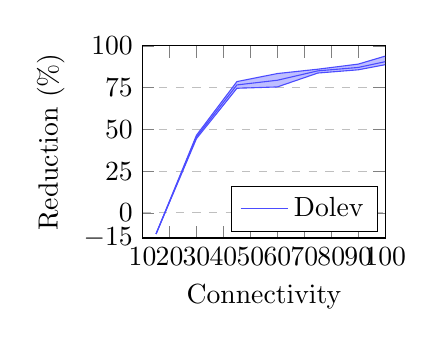
\begin{tikzpicture}
        \begin{axis}[
            xlabel={Connectivity},
            ylabel={Reduction (\%)},
            xmin=10, xmax=100,
            ymin=-15, ymax=100,
            xtick={10,20,30,40,50,60,70,80,90,100},
            ytick={-15,0,25,50,75,100},
            legend pos=south east,
            ymajorgrids=true,
            grid style=dashed,
        ]
        
        \addplot[
            color=blue!70,
            ]
            coordinates {
            (15,-12.59)(30,45.49)(45,76.59)(60,79.40)(75,85.01)(90,87.05)(105,92.23)(120,92.45)(135,93.46)(150,94.39)(165,96.31)
            };
        \addplot[
            name path=dolev_up,
            color=blue!70,
            ]
            coordinates {
            (15,-12.59)(30,46.49)(45,78.59)(60,83.40)(75,86.01)(90,89.05)(105,96.23)(120,94.45)(135,96.46)(150,97.39)(165,97.41)
            };
        \addplot[
            name path=dolev_down,
            color=blue!70,
            ]
            coordinates {
            (15,-12.59)(30,44.49)(45,74.59)(60,75.40)(75,83.71)(90,85.65)(105,90.23)(120,91.2)(135,91.46)(150,93.1)(165,94.31)
            };
        \addplot[blue!50,fill opacity=0.5] fill between[of=dolev_up and dolev_down];
        \addlegendentry{Dolev}
        \end{axis}
        \end{tikzpicture}
    \caption{Reduction using K-random graphs and fully-connected graphs (Bracha)}
    \label{eval:overal-reduction}
\end{figure}

\subsection{Scalability}
In real deployments networks will likely scale quickly, which is why we also evaluated the scalability of the protocol for an increasing number of processes. We considered graphs which include 25 to 150 processes in increments of 25. The connectivity $k$ and Byzantine parameter $f$ are defined as $k=\floor{\frac{N}{3}}$ and $f=\floor{\frac{k-1}{2}}$. The other configuration is identical to the previous sections.

TODO: small eval on scalability.

\begin{figure}[h]
    \centering
    
    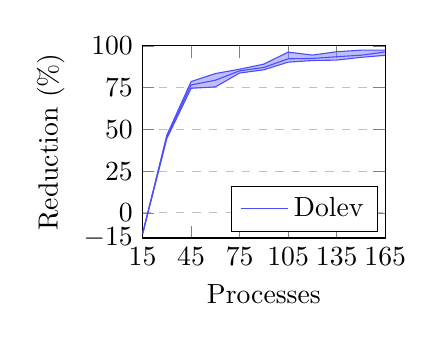
\begin{tikzpicture}
        \begin{axis}[
            xlabel={Processes},
            ylabel={Reduction (\%)},
            xmin=15, xmax=165,
            ymin=-15, ymax=100,
            xtick={15,45,75,105,135,165},
            ytick={-15,0,25,50,75,100},
            legend pos=south east,
            ymajorgrids=true,
            grid style=dashed,
        ]
        
        \addplot[
            color=blue!70,
            ]
            coordinates {
            (15,-12.59)(30,45.49)(45,76.59)(60,79.40)(75,85.01)(90,87.05)(105,92.23)(120,92.45)(135,93.46)(150,94.39)(165,96.31)
            };
        \addplot[
            name path=dolev_up,
            color=blue!70,
            ]
            coordinates {
            (15,-12.59)(30,46.49)(45,78.59)(60,83.40)(75,86.01)(90,89.05)(105,96.23)(120,94.45)(135,96.46)(150,97.39)(165,97.41)
            };
        \addplot[
            name path=dolev_down,
            color=blue!70,
            ]
            coordinates {
            (15,-12.59)(30,44.49)(45,74.59)(60,75.40)(75,83.71)(90,85.65)(105,90.23)(120,91.2)(135,91.46)(150,93.1)(165,94.31)
            };
        \addplot[blue!50,fill opacity=0.5] fill between[of=dolev_up and dolev_down];
        \addlegendentry{Dolev}
        \end{axis}
        \end{tikzpicture}
    \caption{Reduction using K-random graphs and fully-connected graphs (Bracha)}
\end{figure}

\subsection{Discussion}
% Results can be compared to known results and placed in a broader context.
% Provide a reflection on what has been concluded and how this was done.
% Then give a further possible explanation of results.

% You may give this section another name, or merge it with the one before or the one hereafter.
While our results are promising, we have focused on two main statistics: message complexity and network usage. This means that other statistics such as latency have sometimes been sacrificed in order to enhance our chosen statistics, as is the case with \textbf{ORD.6} and \textbf{ORBD.2} for example. This might not be desired in some systems.

We can safely conclude that we can indeed reduce the amount of messages when leveraging topology knowledge, but the system model might be too strict for modern networks as they are generally dynamic instead of static. 

\section{Responsible Research}
% Reflect on the ethical aspects of your research and discuss the reproducibility of your methods.

% \section{Discussion}
% Results can be compared to known results and placed in a broader context.
% Provide a reflection on what has been concluded and how this was done.
% Then give a further possible explanation of results.

% You may give this section another name, or merge it with the one before or the one hereafter.

\section{Conclusion and Future work}
\label{conclusion}
% Summarize the research question(s) and the answers to the research question(s).
% Make statements.
% Highlight interesting elements.

% Discuss open issues, possible improvements, and new questions that arise from this work; formulate recommendations for further research.

% ideally, this section can stand on its own: it should be readable without having read the earlier sections.
In this paper, we have introduced the Byzantine Reliable Broadcast problem on partially connected networks and fully connected networks where the topology is known to all processes. We started by introducing the current state of the problem and how the original protocols work. We continued by elaborating on how one can find the required paths through the network for Dolev, and then how this information can be used to build routing tables for processes. We then described \textbf{9} modifications to Dolev, Bracha, and Bracha-Dolev, and evaluated each modification separately. When we combine all modifications together, we provide a solution with a lower message complexity and network usage than existing solutions, a reduction of 71.9\% and 79.4\% respectively with a 12B payload when $N=150$ and $f=20$ for Dolev.
We have concluded that we can indeed reduce the number of messages transmitted when processes have topology knowledge.

This work can be extended in the future by deploying our modified protocols on real infrastructure to get accurate measurements as opposed to simulations. Furthermore, the disjoint path solver can likely be further optimized by enhancing the path finding and (re)using better suited data structures. Applying our modifications to dynamic networks should also be researched further. In addition to this, we use several simple heuristics in our paper (\textbf{ORB.2}, \textbf{ORD.5}) which should be replaced by optimal solutions or improved heuristics. Another interesting direction is that of topology discovery~\cite{topology-discovery,explorer,explorer2}. Previously unknown networks can use optimizations specific for known networks when matched with a topology discovered. One challenge to overcome in this scenario is the tolerance for imperfect routing tables.

%It might also be interesting to explore the combination of our modifications and (multi-)signatures to further reduce the amount of messages transmitted.


\bibliographystyle{IEEEtran}
\bibliography{references}

\appendix
\section{The obvious}
\subsection{Reference use}
\begin{itemize}
\item use a system for generating the bibliographic information automatically from your database, e.g., use BibTex and/or Mendeley, EndNote, Papers, or \ldots
\item all ideas, fragments, figures and data that have been quoted from other work have correct references
\item literal quotations have quotation marks and page numbers
\item paraphrases are not too close to the original
\item the references and bibliography meet the requirements
\item every reference in the text corresponds to an item in the bibliography and vice versa
\end{itemize}

\subsection{Structure}
Paragraphs
\begin{itemize}
\item are well-constructed
\item are not too long: each paragraph discusses one topic
\item start with clear topic sentences
\item are divided into a clear paragraph structure
\item there is a clear line of argumentation from research question to conclusions
\item scientific literature is reviewed critically
\end{itemize}

\subsection{Style}
\begin{itemize}
\item correct use of English: understandable, no spelling errors, acceptable grammar, no lexical mistakes 
\item the style used is objective
\item clarity: sentences are not too complicated (not too long), there is no ambiguity
\item attractiveness: sentence length is varied, active voice and passive voice are mixed
\end{itemize}

\subsection{Tables and figures}
\begin{itemize}
\item all have a number and a caption
\item all are referred to at least once in the text
\item if copied, they contain a reference
\item can be interpreted on their own (e.g. by means of a legend)
\end{itemize}



\end{document}

